\documentclass[tikz,border=5pt]{standalone}
\usepackage{tikz}
\usetikzlibrary{calc}

\begin{document}
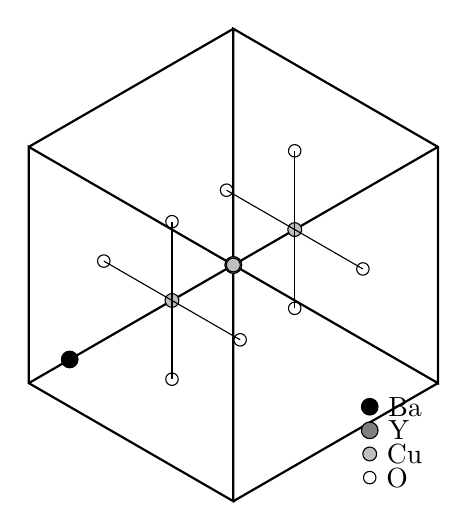
\begin{tikzpicture}[
  scale=1.0,
  x={(0.866cm,-0.5cm)},
  y={(0cm,1cm)},
  z={(0.866cm,0.5cm)}
]

% 原子スタイル
\tikzset{
  Ba/.style={circle, fill=black, draw=black, minimum size=6pt, inner sep=0pt},
  Y/.style={circle, fill=gray, draw=black, minimum size=6pt, inner sep=0pt},
  Cu/.style={circle, fill=gray!50, draw=black, minimum size=5pt, inner sep=0pt},
  O/.style={circle, fill=white, draw=black, minimum size=4.5pt, inner sep=0pt}
}

% ===== 単位胞の枠線 =====
\def\a{3}
\def\b{3}
\def\c{3}
\foreach \z in {0, \c} {
  \draw[thick] (0,0,\z) -- (\a,0,\z) -- (\a,\b,\z) -- (0,\b,\z) -- cycle;
}
\foreach \x/\y in {0/0, \a/0, \a/\b, 0/\b} {
  \draw[thick] (\x,\y,0) -- (\x,\y,\c);
}

% ===== 原子配置(1単位胞)=====
% Ba 原子(上下)
\node[Ba] at (0.3,0.3,0.3) {};
\node[Ba] at (2.7,2.7,0.3) {};

% Y 原子(中心)
\node[Y] at (1.5,1.5,1.5) {};

% Cu 原子(面中心と中央)
\node[Cu] at (1.5,1.5,0.6) {};
\node[Cu] at (1.5,1.5,1.5) {};
\node[Cu] at (1.5,1.5,2.4) {};

% O 原子(平面内)
\foreach \x/\y/\z in {
  1.5/0.5/0.6, 1.5/2.5/0.6, 0.5/1.5/0.6, 2.5/1.5/0.6,
  1.5/0.5/2.4, 1.5/2.5/2.4, 0.5/1.5/2.4, 2.5/1.5/2.4
} {
  \node[O] at (\x,\y,\z) {};
}

% ===== 原子結合(代表) =====
\foreach \dx/\dy in {-1/0, 1/0, 0/-1, 0/1} {
  \draw[thin] (1.5,1.5,0.6) -- ++(\dx,\dy,0);
  \draw[thin] (1.5,1.5,2.4) -- ++(\dx,\dy,0);
}

% ===== 凡例 =====
\begin{scope}[shift={(5,1)}]
  \node[Ba,label=right:Ba] at (0,1.2,0) {};
  \node[Y,label=right:Y] at (0,0.9,0) {};
  \node[Cu,label=right:Cu] at (0,0.6,0) {};
  \node[O,label=right:O] at (0,0.3,0) {};
\end{scope}

\end{tikzpicture}
\end{document}